% status: 100
% chapter: Edge Computing 
% 


\def\paperstatus{100} % a number from 0-100 indicating your status. 100
                % means completed
\def\paperchapter{Edge Computing} % This section is typically a single keyword 
                   % from a small list. Consult with theinstructors about
                   % yours. They typically fill it out once your first
                   % text has been reviewed.
\def\hid{hid-sp18-711} % all hids of the authors of this
                                % paper. The paper must only be in one
                                % authors directory and all other
                                % authors contribute to it in that
                                % directory. That authors hid must be
                                % listed first
\def\volume{10} % the volume of the proceedings in which this paper is to
           % be included

\def\locator{%
	\hid, Volume: \volume, Chapter: \paperchapter, Status: \paperstatus. \newline}


\title{Face Detection and Recognition Using Raspberry Pi Robot Car}

\author{Mani Kumar Kagita}
\affiliation{%
  \institution{Indiana University}
  \streetaddress{107 S. Indiana Avenue}
  \city{Bloomington} 
  \state{Indiana} 
  \postcode{43017-6221}
}
\email{mkagita@iu.edu}

% The default list of authors is too long for headers}
\renewcommand{\shortauthors}{Mani Kumar Kagita}

\begin{abstract}
Face recognition is an exciting and emerging field of computer vision with 
many applications to hardware and devices. Using embedded platforms like 
the Raspberry Pi, a camera module, and an open source computer vision 
library like OpenCV, the purpose is to support face detection to Robot car 
and also face recognition using free developer version of Kairos face 
recognition software.
In today`s modern world, face recognition playing an important role for the 
purpose of security and surveillance and hence there is a need for an 
efficient and cost-effective system. So the main goal is to explore the 
feasibility of implementing Raspberry Pi based face recognition system using 
conventional face detection and recognition techniques such as Haarcascade 
detection and Kairos. An obstacle avoidance robot car is integrated with 
Raspberry Pi and a camera module aiming at taking face recognition to a level 
in which the system can identify the humans who are stuck in buildings during 
earthquakes. Raspberry Pi kit provides the system cost effective and easy to 
use, with high performance.

\end{abstract}


\keywords{Raspberry Pi, Robot Car, Face Recognition, Face Identification, 
	I523, HID319, SP18-711}

\maketitle

\section{Introduction}
A Computer Vision application which has always encouraged people, concern 
about the capability and capacity of robots and computers to determine, 
detect, recognize and interact with human beings~\cite{Boris2014}. We will 
prevail the advantage of cheaper tools that are available in the market for 
computing and detecting a human face from the image, recognizing the face 
using hardware like Raspberry Pi and a video camera that is dedicated to 
Raspberry Pi. Simple and open source software like OpenCV is used to detect 
a human face from the video that is being captured and the image will be 
sent to Kairos face recognition software which allows a high-level approach 
to this process.

In this fastest information era, every information is travelled in a split 
of a second. There is much more need for accurate and fastest methods for 
identifying, recognizing and authentication of humans. In the present world, 
face recognition had become most important and crucial form of human 
identification methods. As per Literature survey statistics in face 
recognition, the two trends to receive significant attention for the past 
several years are; the first is the law enforcement applications and also a 
wide range of commercial techniques, and the second is exponential booming 
of applications and feasible technologies after 30 years of 
research~\cite{riddhi2013}.

The aim is achieved by a possibility to locate human beings or identities 
like faces from the live video capture and within the context of the picture. 
Most advanced human detection applications have this functionality already 
available. When the picture is captured and loaded into the system, it will 
scan the picture and will look for human faces in it. The current 
implementation is to detect face and register them with a name.
If the face is detected and not recognized, Robot car will ask to register 
the detected face with a name. If the human is already registered in Kairos, 
then once the face is detected, Robot car will greet the human with the 
associated name.This whole process determines the Face detection and Face 
recognition techniques using Raspberry Pi and Robot car.

Facial biometric data is to be computed first in creating a complete 
recognition system. This biometric data is then compared with the face 
database and to associate with the human identity. The difference between 
a human and machine is, a human can easily and quickly identify 
characteristics of a human face but then can only save few hundreds of faces. 
Whereas a machine or computers prevails at storing and mapping human 
characteristics and meta data. In the current generation, facial recognition 
software can identify a human face within millions of images from the 
database in seconds. Humans tend to forget human faces as time pass by. 
Machines store them forever. Most of the Law firms across the world follow the 
process and spend huge money on the development of these facial recognition 
systems that can easily identify criminals in real-time. A well-known example 
is studying human faces in airports and bus stations.

The design of the Robot car integrated with Face recognition system will 
navigate through dangerous or natural disaster locations where humans 
unable to enter. Robot car while avoiding obstacles on its way, will 
continuously monitor for human faces who got stuck or in danger and will 
recognize the faces based on the user database. Once the human face is 
recognized, it will intimate to corresponding authorities about the human 
and will help in guiding assistance. 

\section{Face Detection}
Face Detection is a technique referred to computer vision technology which 
is able to identify human faces within digital images~\cite{divya2013}. Face 
detection applications work using algorithms and machine learning formulas 
for detecting human faces in the visual images. Identifying only human faces 
from these images which can contain landscapes, houses, animals is called 
Face Detection technique.

Face Detection is termed to only identify if there are any humans present in 
the image or a video. It lacks the inability to recognize which human face is 
present. Common widely used face detection techniques are in auto-focus of a 
digital camera. During auto-focus, camera lens will look for human faces in 
the range and identify them to have focus in that particular area.
Face Detection techniques will be widely used in counting how many numbers 
of visitors attending a particular event.

\subsection{How Face Detection Works}
While Face Detection process is somewhat complex, the algorithms will start 
off by searching for human eyes at first. Eyes usually represent a valley 
region and its the easiest feature in human face to detect. Once the eyes 
are detected, then the algorithms will look for rest of the characteristics 
of a human face such as iris, nose, mouth, eyebrows, and nostrils. 
Face detection algorithm then summarizes the data and shows that it has 
successfully detected a human face from the facial region. Additional tests 
can be conducted by the algorithm to make sure and validate if the human face 
is detected~\cite{jesse2017}.

\section{Face Recognition}
Like most of the biometric solutions, face recognition technology will be 
used for identification and authentication purposes by measuring and matching 
the unique facial characteristics of a human face. Using a digital camera 
connected to the Raspberry Pi, once the face is detected, face recognition 
software will quantify the characteristics of face and then will match with 
the stored images in the database. Once the match is positive, then the 
corresponding name will be displayed as output~\cite{biometrics2016}.

Facial biometrics can be integrated with any system having a camera. Border 
control agencies use face recognition to verify identities of the travellers 
and can separate them from the trespassers. Government Law agencies replace 
all the security cameras around the world with biometric applications to scan 
faces in CCTV footage and to identify persons of interest in the field. Face 
recognition has become one of the fastest and human un-intervention techniques 
to find out the identity of a particular human~\cite{biometrics2016}.

For the past few years, Face recognition has become one of the most commonly 
used biometric authentication techniques. It mainly deals with the pattern 
recognition and analysing the images. Two main tasks of face recognition 
are: Face Verification and Face Identification. Face Verification is 
comparing a human face in an image with a template image and recognizing 
the correct patterns. Face Identification is comparing human face in an 
image with multiple images in the database. Face recognition techniques 
have more advantages than any other biometrics. With well-sophisticated 
algorithms and coding, face recognition has a high recognition rate or high 
identification rate of more than 90\%~\cite{riddhi2013}.

\begin{figure}[!ht]
  \centering
  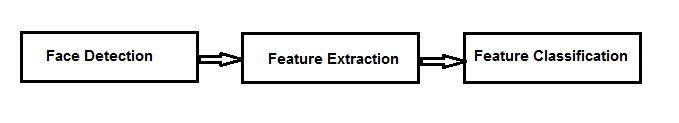
\includegraphics[width=\columnwidth]{images/Face-recognition.jpg}
  \caption{Block Diagram of a Face Recognition System}
\end{figure}

\subsection{Face Recognition and Big Data Analysis}

Face Recognition and Big Data are two distinct technologies which are 
having hardly anything in common. But when they both are put together, 
a technology drift takes place in terms of biometric authentication. 
Storing a massive unique characteristics and libraries of human faces, 
algorithms are used to run on these characteristics to recognize the 
human face accurately. Using big data, a real-time analysis can be done 
which identifies faces and applies the rules as they are happening.

Robot car is designed to collect all the facial features that are encountered 
on its path and store them in the cloud. When the face is detected by the 
camera, it sends the picture to the cloud and facial recognition software 
will compare with huge database of faces that are located in the cloud. 
Once the face features match, robot car will respond with the unique name 
that is set for that human face.

\section{Software and Hardware Specifications}
OpenCV is to be installed in Raspberry Pi to detect human faces within the 
captured images. Kairos face recognition software is used to recognize a 
human face and identify with the corresponding name.

\subsection{Software Used}

\subsubsection{Raspbian OS}
This is the recommended OS for Raspberry Pi 3. Raspbian OS is Debian based 
operating system. It can be installed from NOOBS installer. Raspbian comes 
with various pre-installed software such as Python, Sonic Pi, Java, 
Mathematica for programming and education.

\subsubsection{Putty}
PuTTY is an SSH and telnet client for the Windows platform. PuTTY is open 
source software that is available with source code and is developed and 
supported by a group of volunteers. Here we are using putty for accessing 
our Raspberry Pi remotely.

\subsubsection{OpenCV}
OpenCV (Open Source Computer Vision Library) is an open source computer 
vision and machine learning software library. OpenCV was built to provide 
a common infrastructure for computer vision applications and to accelerate 
the use of machine perception in the commercial products. Being a 
BSD-licensed product, OpenCV makes it easy for businesses to utilize and 
modify the code. The library has more than 2500 optimized algorithms, 
which includes a comprehensive set of both classic and state-of-the-art 
computer vision and machine learning algorithms. These algorithms can be 
used to detect and recognize faces, identify objects, classify human 
actions in videos, track camera movements, track moving objects and extract 
3D models of objects~\cite{opencv}.

\subsubsection{Python 2 IDE}
Python 2.7.x version Integrated Development Environment is used to compile 
python program in Raspberry Pi. IDE is a text editor plus terminal 
combination which is used to work on large projects with complex code bases.

\subsubsection{Kairos Face Recognition Software}
Kairos is an artificial intelligence company specializing in face recognition. 
Through computer vision and machine learning, Kairos can recognize faces in 
videos,photos, and the real-world. A captured image is sent to Kairos using 
an API call and then Kairos will search with the face database. If it matches 
then will reply with the human name.

\begin{itemize}
\item Identity
\item Emotions
\item Demographics
\end{itemize}

Kairos navigates the complexities of face analysis technology.

\subsection{Hardware Used}
\subsubsection{Raspberry Pi 3}
Raspberry Pi 3 is the latest version of Raspberry Pi. Unless previous 
versions, this have an inbuilt Bluetooth platform and a wifi support 
module. There are total 40 pins in RPI3. Of the 40 pins, 26 are GPIO 
pins and the others are power or ground pins (plus two ID EEPROM pins). 
There are 4 USB ports, 1 Ethernet slot, one HDMI port, 1 audio output port 
and 1 micro USB port. And also we have one micro SD card slot wherein we 
have to install the recommended operating system on the micro SD card. 
There are two ways to interact with your Raspberry Pi. Either you can 
interact directly through HDMI port by connecting HDMI to VGA cable, and 
keyboard and mouse or else you can interact from any other system through 
SSH (Secure Shell)~\cite{deligence2017}.

\subsubsection{Raspberry Pi Camera}
The Raspberry Pi camera module can be used to take high-definition video, 
as well as stills photographs. It`s easy to use for beginners but has 
plenty to offer advanced users if you’re looking to expand your knowledge. 
There are lots of examples online of people using it for time-lapse, 
slow-motion and other video cleverness. You can also use the libraries we 
bundle with the camera to create effects.

\subsubsection{Robot Car Chassis Kit}
The Mechanical design of the Robot car includes hardware such as motor and 
wheel placement and body set-up. Robot car uses two gear-motors attached to 
wheels and one free-wheel for having various movements like forward, 
backward, left and right. Free-wheel ball is placed at the rear side of the 
robot which helps for 360 degrees free movement~\cite{arduino2015}. L298N 
DC Stepper Motor Drive controller is used to control the speed and direction 
of the two gear motor wheels. Ultrasonic sensors are placed on the front 
side of the robot which is capable to detect the objects on its 
path~\cite{gregor2017}.



\section{System Architecture}
System Architecture consists of following blocks:

\begin{itemize}
\item[a.] Raspberry Pi
\item[b.] Raspberry Pi Camera Module
\item[c.] L298N Dual H-Bridge Stepper Motor Controller
\item[d.] DC power supply 12v and 5v
\item[e.] Robot Car chassis kit
\item[f.] HC-SR04 Ultrasonic Sensor
\item[g.] SG90 Servo Motor.
\item[h.] Wires, Breadboard, Small PCB.
\end{itemize}


\section{Setup}
\subsection{Connect Raspberry Pi}
This section includes connectivity of Raspberry Pi to wifi. 

\begin{itemize}
\item Download Raspbian operating system to an SD card with a minimum 
capacity of 8GB.
\item Plugin USB power cable, keyboard, mouse and monitor cables to 
Raspberry Pi. 
\item Insert the SD card with Raspbian OS into Pi and boot the system. 
Once the Pi is booted up, a window will appear with the Raspbian 
operating system. Click on Raspbian and Install.
\item Once the install process has completed, the Raspberry Pi configuration 
menu (raspi-config) will load. Here set the time and date for your region.
\item Enable wifi located at the upper right corner of the desktop and connect 
to wifi sid.
\end{itemize}


\subsection{Connect Raspberry Pi Camera Module}
Before setting the camera configurations, first connect the camera to 
Raspberry Pi. The cable slots into the connector situated between the 
Ethernet and HDMI ports, with the silver connectors facing the HDMI port. 
Once the connection is completed, boot up the Raspberry Pi and run the 
following commands to install various supporting libraries. 
Skip first two steps if Python is already installed on Raspberry Pi.

\begin{itemize}
\item sudo apt-get install python-pip
\item sudo apt-get install python-dev
\item sudo pip install picamera
\item sudo pip install rpio
\end{itemize}

Once the libraries are installed, follow below steps to check if camera 
is installed in Raspberry Pi.
\begin{itemize}
\item sudo raspi-config
\end{itemize}


If the camera option is not listed in the options, run the following commands 
to update Raspberry Pi.
\begin{itemize}
\item sudo apt-get update
\item sudo apt-get upgrade
\end{itemize}

\subsubsection{Enable Camera}
For face detection, PiCamera should be enabled from Raspberry Pi. The 
following list of figures shows the detailed steps on how to enable PiCamera.

As shown in Figure~\ref{F:raspi}, execute the configuration command from 
terminal. From the listed options, select ``Enable Camera'' as shown in 
Figure~\ref{F:selcamera}. Click on ``Yes'' option to enable the camera 
interface as shown in Figure~\ref{F:enbcamera}.

\begin{figure}[!ht]
  \centering
  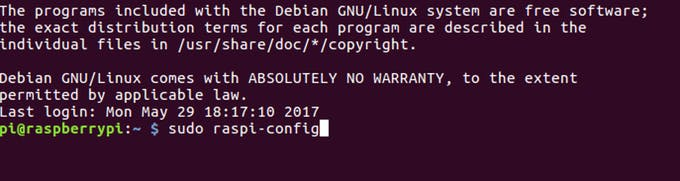
\includegraphics[width=\columnwidth]{images/enablecamera1.jpg}
  \caption{Execute raspi config from command line terminal}\label{F:raspi}
%\end{figure}

\bigskip

%\begin{figure}
  \centering
  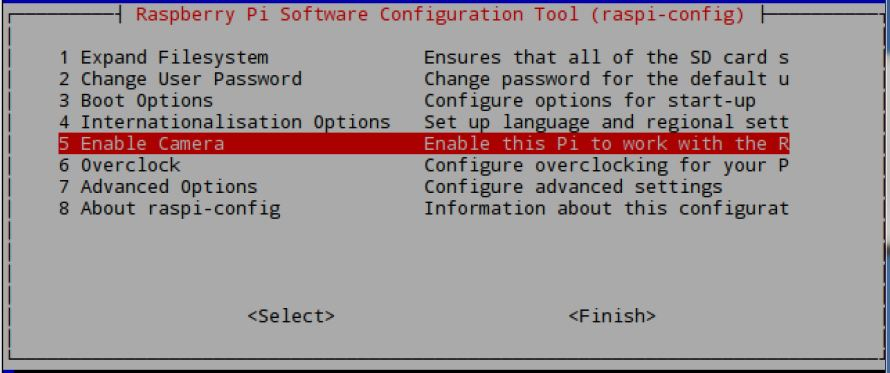
\includegraphics[width=\columnwidth]{images/enablecamera2.jpg}
  \caption{Select Camera from the options}\label{F:selcamera}
%\end{figure}

\bigskip

%\begin{figure}
  \centering
  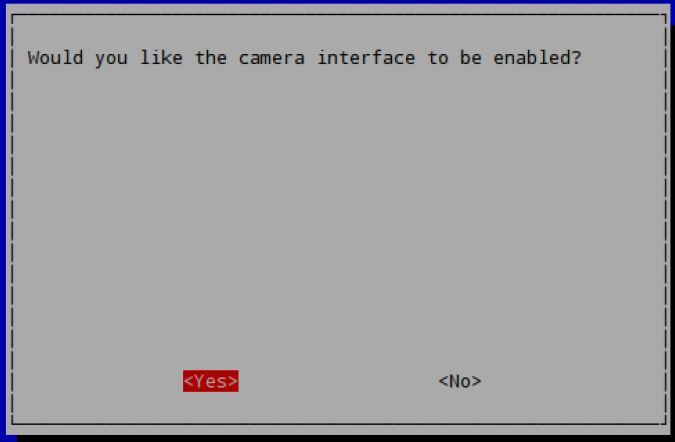
\includegraphics[width=\columnwidth]{images/enablecamera3.jpg}
  \caption{Enable Camera}\label{F:enbcamera}
\end{figure}

\subsection{Install OpenCV and Required Libraries}
OpenCV computer vision library is used to for face detection from the live 
video streaming. Execute the following commands to install OpenCV dependencies 
on the Raspberry Pi.

\begin{verbatim}
sudo apt-get install build-essential
sudo cmake pkg-config python-dev libgtk2.0-dev \
		libgtk2.0 zlib1g-dev libpng-dev \
		libjpeg-dev libtiff-dev libjasper-dev \
		libavcodec-dev swig unzip
\end{verbatim}
Select yes for all options and wait for the libraries and dependencies to be 
installed.


Download opencv-2.4.9 zip file to Raspberry Pi. Change to the corresponding 
directory and execute the following commands.

\begin{verbatim}
cd opencv-2.4.9
sudo apt-get install build-essential cmake \
		pkg-config
sudo apt-get install libjpeg-dev libtiff5-dev \
		libjasper-dev libpng12-dev
sudo apt-get install python-dev python-numpy \
		libtbb2 libtbb-dev libjpeg-dev \
		libpng-dev libtiff-dev libjasper-dev \
		libdc1394-22-dev
sudo apt-get install python-opencv
sudo apt-get install python-matplotlib

\end{verbatim}

After executing the commands the latest version of OpenCV is now installed 
in Raspberry Pi. Time taken to install OpenCV is about 15 minutes.

\subsection{Integration of Raspberry Pi with Robot Car}
Raspberry Pi connected with PiCamera is integrated with Robot car to navigate 
using a web server. During the navigation, robot car will look for human 
faces using PiCamera and then detects the face. Once the face is detected, 
python program will call Kairos face detection software to identify the 
person and greet with the name. If the human face is unidentified then robot 
car will ask human to register their name.
The diagram in Figure~\ref{F:circuit} shows the circuit connections of 
Raspberry Pi to stepper motor controller and DC motors of a robot car.

\begin{figure}[htb]
  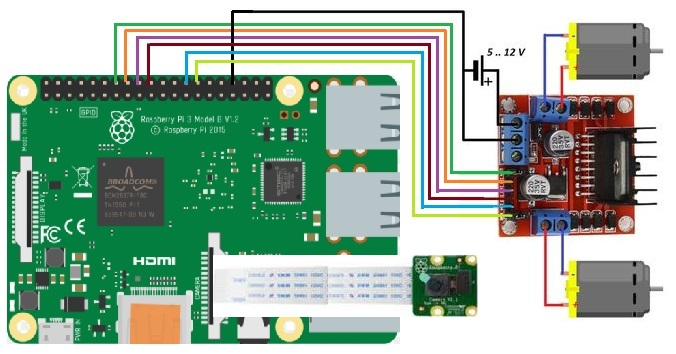
\includegraphics[width=1.0\columnwidth]{images/RaspPi_Robot.jpg}
  \caption{Raspberry Pi Robot Car Integration}\label{F:circuit}
\end{figure}

Figures~\ref{F:robotfront},~\ref{F:robotside},~\ref{F:robottop}  represents 
corresponding front view, sideview and topview of the robot car connections.

\begin{figure}[htb]
  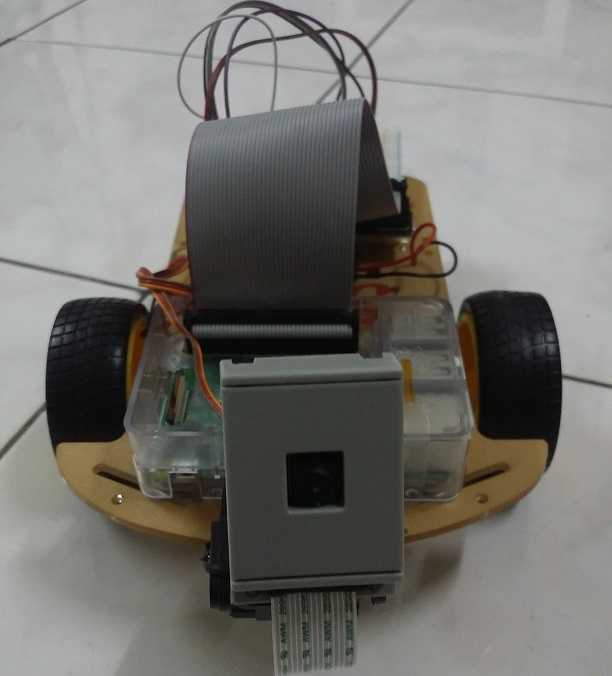
\includegraphics[width=0.8\columnwidth]{images/RobotCar_FrontView.jpg}
  \caption{Front view of Robot Car}\label{F:robotfront}
%\end{figure}

%\begin{figure}
  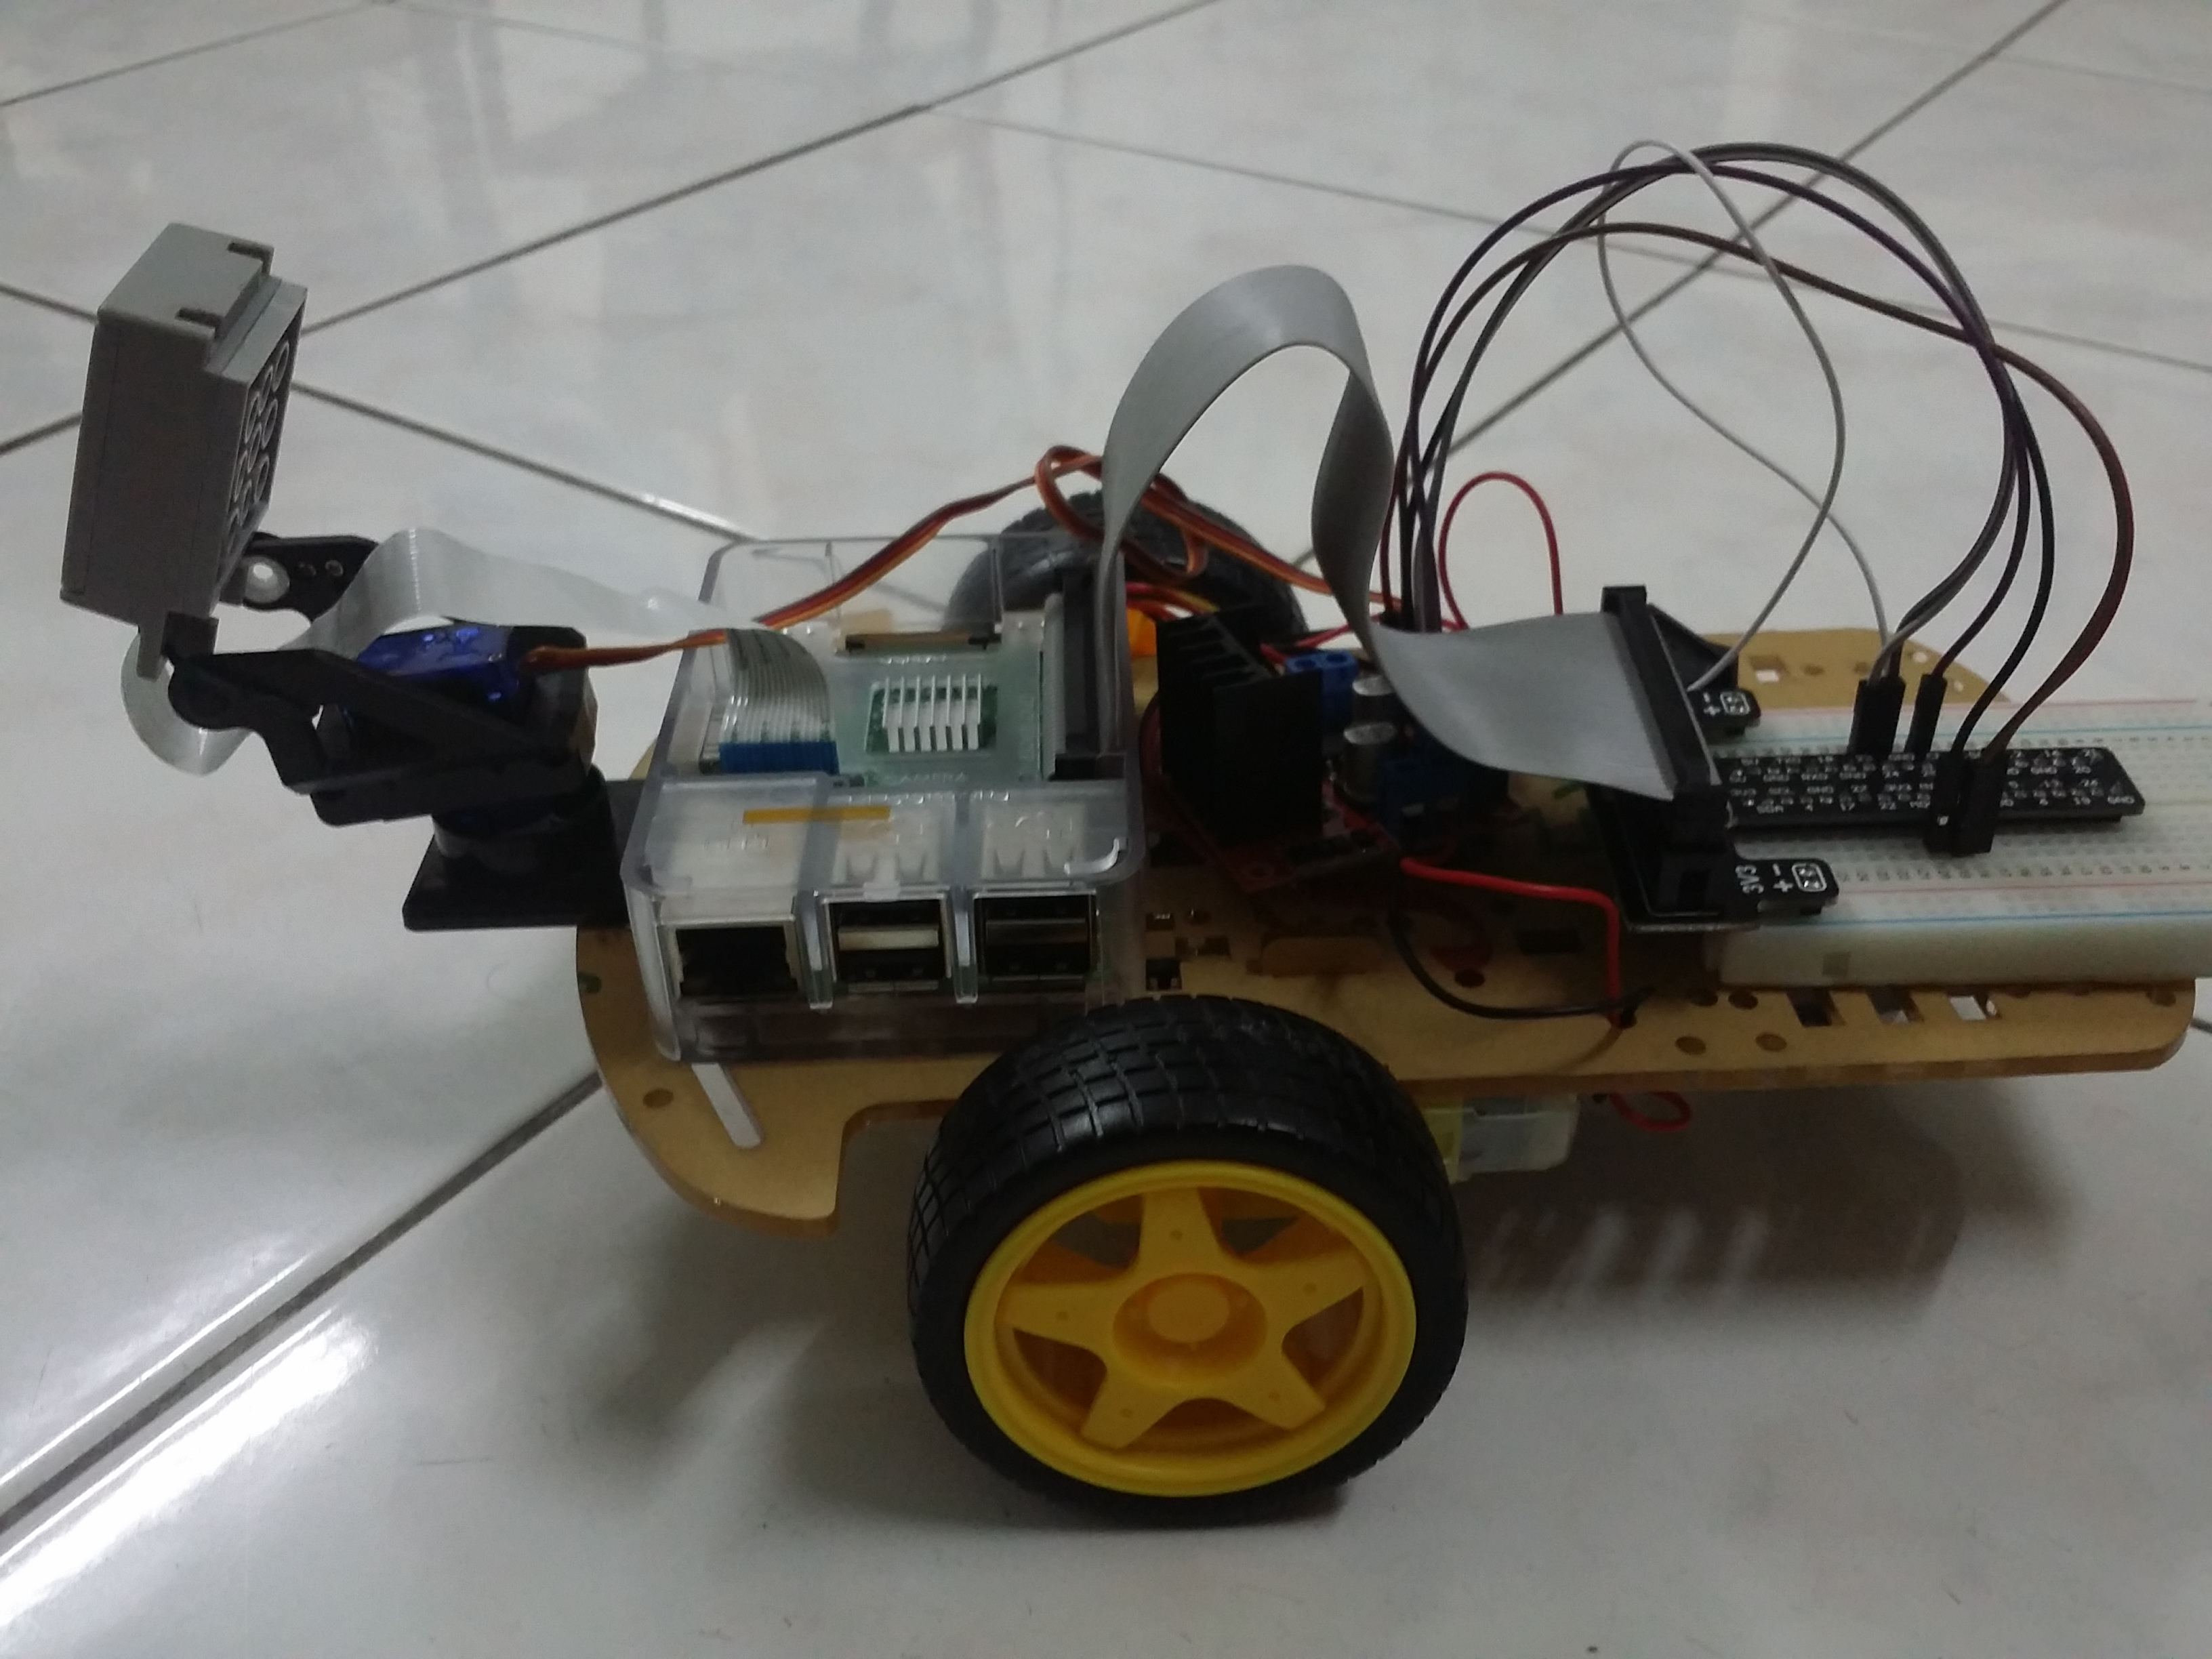
\includegraphics[width=0.8\columnwidth]{images/RobotCar_SideView.jpg}
  \caption{Side view of Robot Car}\label{F:robotside}
%\end{figure}

%\begin{figure}
  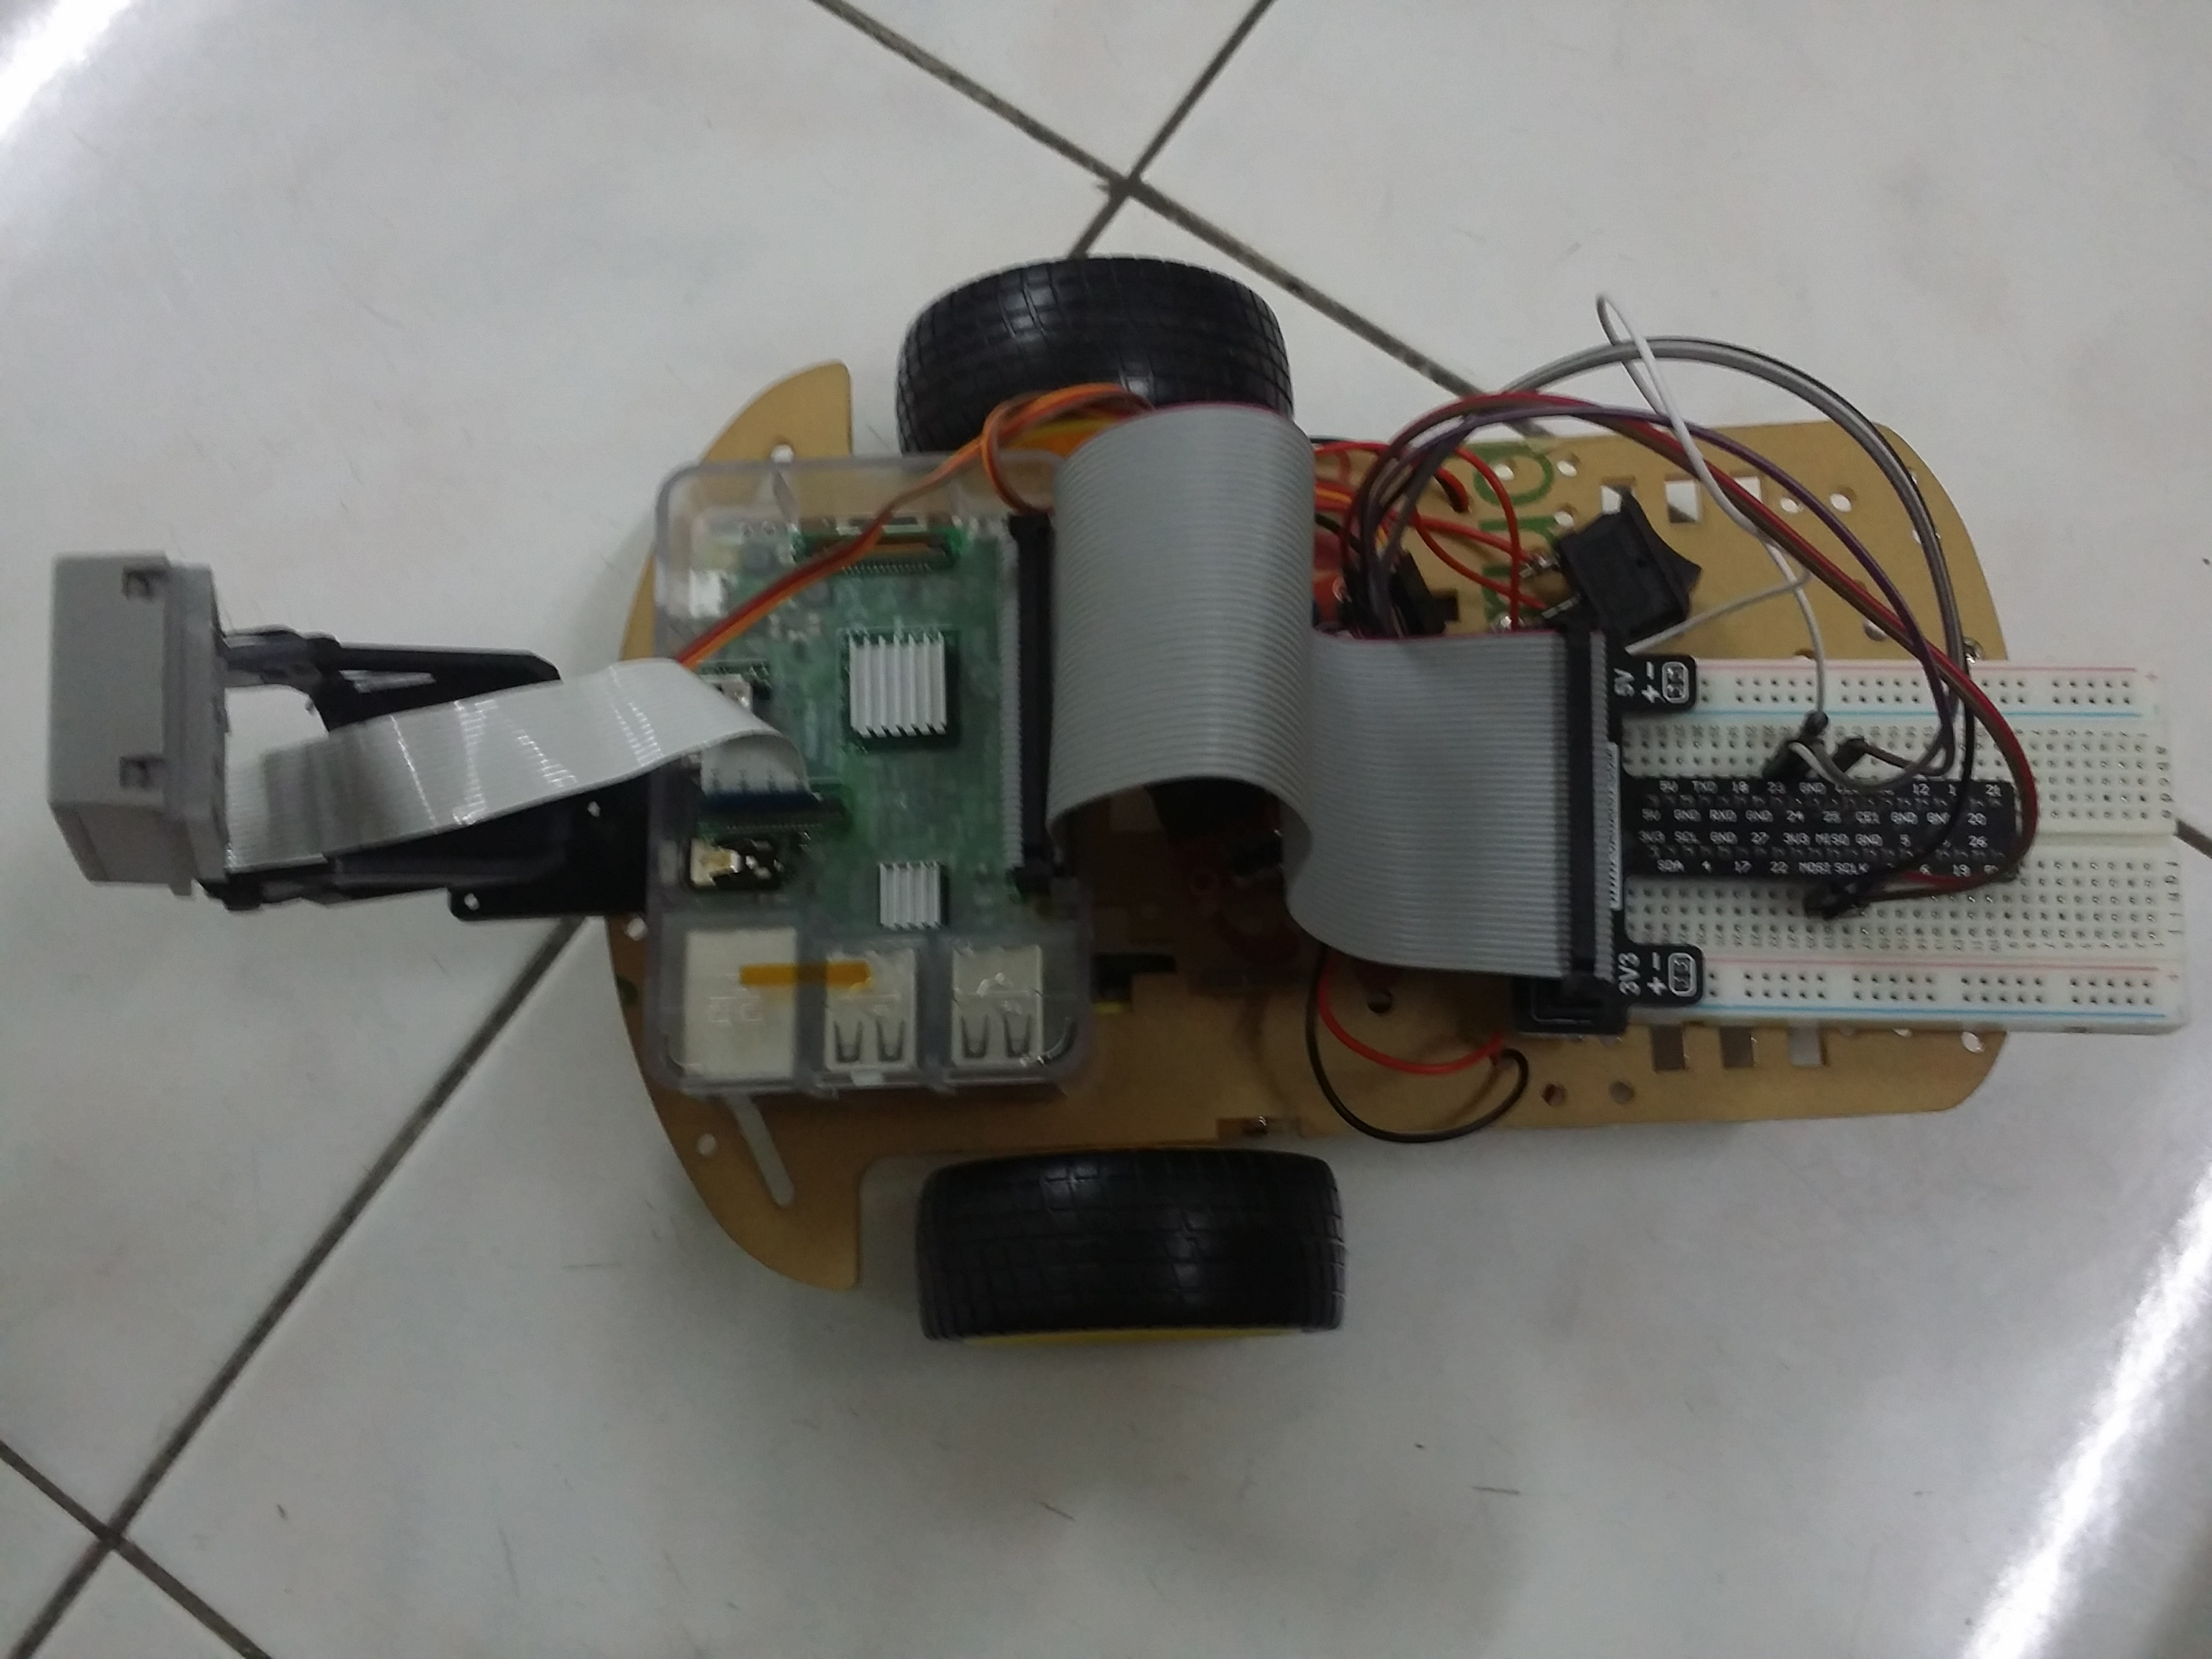
\includegraphics[width=0.8\columnwidth]{images/RobotCar_TopView.jpg}
  \caption{Top view of Robot Car}\label{F:robottop}
\end{figure}


In the Table~\ref{T:pinlayout}, shows the connectivity of Raspberry Pi GPIO 
pins to L298N stepper motor controller.

\begin{table}[htb]
\caption{Pin connections of Raspberry Pi to stepper motor 
controller}\label{T:pinlayout}
\begin{tabular}{lll}
Actuator & Raspberry Pi GPIO Pin & L298N Pin \\
\hline
    Motor1A & GPIO23 & IN1 \\
    Motor1B & GPIO24 & IN2 \\
    Motor1Enable & GPIO25 & ENA \\
    Motor2A & GPIO9 & IN3 \\
    Motor2B & GPIO10 & IN4 \\
    Motor2Enable & GPIO11 & ENB \\
\end{tabular}
\end{table}


\subsection{Kairos Face Recognition Setup}
Kairos Face Recognition system has a free developer account which is used 
to identify the human name from the images. Once registered a human name 
with an image, the code will call Kairos API with a newly detected human 
face and will look for the registered name. Kairos will do a quick look-up 
in the human database from the registered account and if it matches, will 
send the name of the human back to the code.

Setup as follows:

\begin{itemize}
\item Register with Kairos using url ``https:/www.kairos.com'' as a free 
developer account
\item Login with registered username and password
\item Create an appname
\item An app id and a key will be generated. Save this for future use.
\item Enroll a sample user and a gallery name with the user image using 
following POST request.


    \begin{verbatim}
    POST /enroll HTTP/1.1
    Content-Type: application/json
    app_id: your-app-id
    app_key: your-app-key
    {
    "image":" http://media.kairos.com/user.jpg ",
    "subject_id":"User",
    "gallery_name":"MyGallery"
    }
    \end{verbatim}
\end{itemize}


With the completed steps, Kairos face recognition application will be created 
and ready for face recognition from the images.

\section{Code Explanation}
\subsection{Face Detection}
Before configuring face detection for the robot car, related libraries 
including PiCamera and PiRGBArray libraries for camera to operate should 
be imported in the code. These libraries will help to capture video and 
images from the PiCamera.


\begin{verbatim}
from picamera.array import PiRGBArray
from picamera import PiCamera
import time
import cv2
import sys
import imutils
from fractions import Fraction
import base64
import requests
import json
import random
import os
\end{verbatim}


Haar Feature-based cascade classifier is an effective face or object 
detection method to capture the frontal features of the 
face~\cite{viola2001}. This tool will help to continuous monitoring 
of any human face to detect. Once detected a human face, the output values 
will provide as Human Face Detected from the capturing video.


\begin{verbatim}
# Get user supplied values
cascPath = './haarcascade_frontalface_default.xml'

# Create the haar cascade
faceCascade = cv2.CascadeClassifier(cascPath)
\end{verbatim}


Camera settings need to be updated in the code as per below suggestions. 
The captured image is to be sent to Kairos for face recognition and so we 
will set the resolution to a lower level. This will help to send the image 
faster over the network without any delay.


\begin{verbatim}
# initialize the camera 
#camera capture
camera = PiCamera()
camera.resolution = (160, 120)
camera.framerate = 32
rawCapture = PiRGBArray(camera, size=(160, 120))
\end{verbatim}


Below code represents PiCamera continuously monitor for human faces detected 
from the grayscale video capture. Once the human face is detected, espeak 
function in Raspberry Pi will send the voice to a connected speaker and will 
output as ``Human face detected''. This detected image is then saved as 
``User-Image.jpg'' which is then will be sent to Kairos during Face 
recognition.

Images in Figures~\ref{F:frontview},~\ref{F:sideview1},~\ref{F:sideview2} 
represents face detection of front and side views within the circle using 
OpenCV.


\begin{figure}[htb]
  \centering
  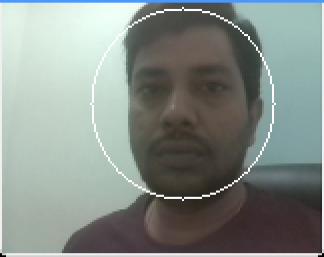
\includegraphics[width=\columnwidth]{images/Face-detect-frontview.png}
  \caption{Front view of Face detection}\label{F:frontview}
%\end{figure}

%\begin{figure}
  \centering
  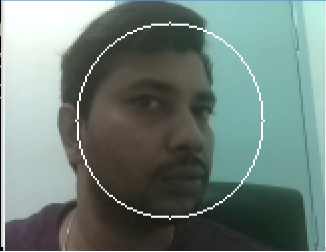
\includegraphics[width=\columnwidth]{images/Face-detect-sideview1.png}
  \caption{Side view 1 Face detection}\label{F:sideview1}
%\end{figure}

%\begin{figure}
  \centering
  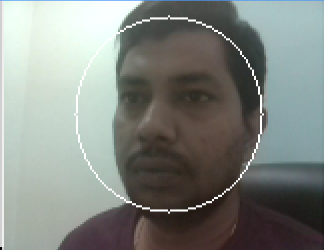
\includegraphics[width=\columnwidth]{images/Face-detect-sideview2.png}
  \caption{Side view 2 Face detection}\label{F:sideview2}
\end{figure}


\begin{verbatim}
# allow the camera to warm-up
time.sleep(0.1)
lastTime = time.time()*1000.0
# capture frames from the camera
for frame in camera.capture_continuous(rawCapture, \ 
	format="bgr", use_video_port=True):
	# grab the raw NumPy array representing the image, 
	# then initialize the timestamp and 
	# occupied/unoccupied text
    image = frame.array
    gray = cv2.cvtColor(image, cv2.COLOR_BGR2GRAY)
    
    # Detect faces in the image
    faces = faceCascade.detectMultiScale(
    	gray,
    	scaleFactor=1.1,
    	minNeighbors=5,
    	minSize=(30, 30),
    	flags = cv2.cv.CV_HAAR_SCALE_IMAGE
    )
    print time.time()*1000.0-lastTime," \
    Found {0} faces!".format(len(faces))
    lastTime = time.time()*1000.0

    # Draw a circle around the faces
    for (x, y, w, h) in faces:
        cv2.circle(image, (x+w/2, y+h/2), \
        int((w+h)/3), (255, 255, 255), 1)
    # show the frame
    cv2.imshow("Frame", image)
    key = cv2.waitKey(1) & 0xFF
    if len(faces) == 1:
        print("Taking image...")
	camera.capture("foo.jpg")
	os.system('espeak "Human face detected"')
	inputImage= "./foo.jpg"
	del camera
	break 
	# clear the stream in preparation for the 
	#next frame
    rawCapture.truncate(0)
    
	# if the `q` key was pressed, break from 
	#the loop
    if key == ord("q"):
        del camera
        exit()
\end{verbatim}


\subsection{Face Recognition}
For the Face Recognition, we use Kairos to detect the facial characteristics. 
A JSON config file is to be placed in the same folder as of the code with 
Kairos API app id and key value. When the human face is detected, the code 
will generate an API call to Kairos software along with the gallery name, 
API app id and key values. Image when sending to Kairos, it will be base64 
encrypted and will send over the network for security purpose. This encrypted 
image will then be decrypted at Kairos platform.


\begin{verbatim}
KAIROS = "api.kairos"
KairosGallery = 'MyFace'
KairosConfig = './kairos_config.json'
\end{verbatim}

\begin{verbatim}
def trainKairos(image, name):
    global KairosGallery
    headers = {
        'app_id': 'your-app-idd39fc1b1',
        'app_key': 'your-app-key'
    }
    data = {
        'image': base64.b64encode(image),
        'gallery_name': KairosGallery,
        'subject_id': name
    }
    r = requests.post('http://api.kairos.com/enroll', \ 
        headers=headers, data=json.dumps(data))
    print(r.text)
    return(None)
\end{verbatim}

\begin{verbatim}
class Recognize():
    def __init__(self, API, config_file):
        self.api = API
        self.config = config_file

    #def recognize(self, image_path):
    #    return self.__recognizeKairos(image_path)
    
    def recognizeKairos(self, image):
        with open(image, "rb") as image_file:
            encoded_string = base64.b64encode\
            (image_file.read())
        with open(self.config, "rb") as config_file:
            config = json.loads \ 
            (config_file.read())
        data = {
            "image": encoded_string,
            "gallery_name": config["gallery_name"]
        }

        headers = {
            "Content-Type": "application/json",
            "app_id": config["app_id"],
            "app_key": config["app_key"]
        }
\end{verbatim}

The output from Kairos software is in JSON format. The output is then 
segregated as per the key-value pairs and then saved into local variables. 
When the image is recognized, a success transaction message will be 
obtained from Kairos along with subject id and face id.

\begin{verbatim}
try:
    r = requests.post("https://api.kairos.com/recognize", \ 
                 headers=headers, data=json.dumps(data))
    data = r.json()
    print data
    # print json.dumps(data, indent=4)
    faces = []
    if "images" in data:
        for obj in data["images"]:
            if obj["transaction"]["status"] == \
            "success":
                face_obj = {}
                face_obj["person"] = \
                obj["transaction"]["subject_id"]\
                .decode("utf_8")
                #face_obj["faceid"] = \
                obj["candidates"][0]["face_id"]\
                .decode("utf_8")
                face_obj["confidence"] = \
                obj["transaction"]["confidence"]
                faces.append(face_obj)
            elif obj["transaction"]["status"] == \
            "failure":
                face_obj = {}
                face_obj["person"] = "unidentified"
                face_obj["confidence"] = 0
                faces.append(face_obj)
            else:
                print "its in last loop"
            return faces
 except requests.exceptions.RequestException as \
 exception:
       print exception
        return None
\end{verbatim}    

The output from Kairos face recognition software is to be read to understand 
if the person name is identified or not. If it is identified then the person 
name will be listed according to the corresponding person in the image. If 
the human is not identified, then the code will suggest if the user wants 
to registered for face recognition. Once the user key in the name, Kairos 
API call is generated while sending newly registered name and the gallery 
name to that corresponding application id. Here the newly recognized user 
will be registered with the name and his image. When the user is recognized 
by the camera in next corresponding events, then Robot car will greet the 
user with his name.

\begin{verbatim}
if __name__ == "__main__":
    r = Recognize(KAIROS, "kairos_config.json")
    x = r.recognizeKairos(inputImage)
    
    #print x
    #print x["person"]
    #print x[0]["person"]
    string1 = x[0]["person"]
    #print string1
    os.system('espeak "Hello...""{}"'.format(string1))
    if x[0]["person"] == "unidentified":
        os.system('espeak "Please enter your \ 
                  name to Register"')
        nameToRegister = raw_input("Please enter \ 
                        your name to Register :")
        binaryData = open(inputImage, 'rb').read()
        print('Enrolling to Kairos')
        trainKairos(binaryData, nameToRegister)
        print "You are now Registered as :", \ 
        nameToRegister os.system('espeak \ 
        "Hello...""{}"'.format(nameToRegister))
        exit()
\end{verbatim}

\subsection{Robot Car Navigation}
\begin{verbatim}
import RPi.GPIO as GPIO
from time import sleep

GPIO.setmode(GPIO.BOARD)
\end{verbatim}

\begin{verbatim}
#Connecting two wheel motors to Raspberry Pi GPIO 
#Left Motor (Motor 1) connections
Motor1A = 16 #(GPIO 23 - Pin 16)
Motor1B = 18 #(GPIO 24 - Pin 18)
Motor1Enable = 22 #(GPIO 25 - Pin 22)

#Right Motor (Motor 2) Connecctions
Motor2A = 21 #(GPIO 9 - Pin 21)
Motor2B = 19 #(GPIO 10 - Pin 19)
Motor2Enable = 23 #(GPIO 11 - Pin 23)
\end{verbatim}

\begin{verbatim}
#Ouptut of Morors to set as OUT
GPIO.setup(Motor1A,GPIO.OUT)
GPIO.setup(Motor1B,GPIO.OUT)
GPIO.setup(Motor1Enable,GPIO.OUT)
GPIO.setup(Motor2A,GPIO.OUT)
GPIO.setup(Motor2B,GPIO.OUT)
GPIO.setup(Motor2Enable,GPIO.OUT)

\end{verbatim}

\begin{verbatim}
# Defining function for Robot car to move forward
def forward():
	GPIO.output(Motor1A,GPIO.HIGH)
	GPIO.output(Motor1B,GPIO.LOW)
	GPIO.output(Motor1Enable,GPIO.HIGH) 
	GPIO.output(Motor2A,GPIO.HIGH)
	GPIO.output(Motor2B,GPIO.LOW)
	GPIO.output(Motor2Enable,GPIO.HIGH) 

	sleep(2)
\end{verbatim}

\begin{verbatim}
# Defining function for Robot car to move backward
def backward():
	GPIO.output(Motor1A,GPIO.LOW)
	GPIO.output(Motor1B,GPIO.HIGH)
	GPIO.output(Motor1Enable,GPIO.HIGH)
	GPIO.output(Motor2A,GPIO.LOW)
	GPIO.output(Motor2B,GPIO.HIGH)
	GPIO.output(Motor2Enable,GPIO.HIGH)

	sleep(2)
\end{verbatim}

\begin{verbatim}
# Defining function for Robot car to turn right
def turnRight():
	print("Going Right")
	GPIO.output(Motor1A,GPIO.HIGH)
	GPIO.output(Motor1B,GPIO.LOW)
	GPIO.output(Motor1Enable,GPIO.HIGH)
	GPIO.output(Motor2A,GPIO.LOW)
	GPIO.output(Motor2B,GPIO.LOW)
	GPIO.output(Motor2Enable,GPIO.LOW)

	sleep(2)
\end{verbatim}

\begin{verbatim}
# Defining function for Robot car to turn left
def turnLeft():
	print("Going Left")
	GPIO.output(Motor1A,GPIO.LOW)
	GPIO.output(Motor1B,GPIO.LOW)
	GPIO.output(Motor1Enable,GPIO.LOW)
	GPIO.output(Motor2A,GPIO.HIGH)
	GPIO.output(Motor2B,GPIO.LOW)
	GPIO.output(Motor2Enable,GPIO.HIGH)

	sleep(2)
\end{verbatim}

\begin{verbatim}
# Defining function for Robot car to stop
def stop():
	print("Stopping")
	GPIO.output(Motor1A,GPIO.LOW)
	GPIO.output(Motor1B,GPIO.LOW)
	GPIO.output(Motor1Enable,GPIO.LOW)
	GPIO.output(Motor2A,GPIO.LOW)
	GPIO.output(Motor2B,GPIO.LOW)
	GPIO.output(Motor2Enable,GPIO.LOW)
\end{verbatim}

\subsection{Controling Robot Car using webserver}
\begin{verbatim}
from flask import Flask, render_template, \ 
request, redirect, url_for, make_response
import RPi.GPIO as GPIO
import motors

#set up GPIO
GPIO.setmode(GPIO.BOARD) 

#set up flask server
app = Flask(__name__) 

#when the root IP is selected, return index.html page
@app.route('/')
def index():

	return render_template('index.html')
\end{verbatim}

\begin{verbatim}
#recieve which pin to change from the button press on \ 
#index.html
#each button returns a number that triggers a command in \ 
#this function
#
#Uses methods from motors.py to send commands to the GPIO \ 
# to operate the motors
@app.route('/<changepin>', methods=['POST'])
def reroute(changepin):

	changePin = int(changepin) #cast changepin to an int

	if changePin == 1:
		motors.turnLeft()
	elif changePin == 2:
		motors.forward()
	elif changePin == 3:
		motors.turnRight()
	elif changePin == 4:
		motors.backward()
	else:
		motors.stop()


	response = make_response(redirect(url_for('index')))
	return(response)

#set up the server in debug mode to the port 8000
app.run(debug=True, host='0.0.0.0', port=8000) 
\end{verbatim}

\section{Applications}
There are lots of applications of face recognition. Face recognition is 
already being used to unlock phones and specific applications. Face 
recognition is also used for biometric surveillance. Banks, retail stores, 
stadiums, airports and other facilities use face recognition to reduce 
crime and prevent violence.

\section{Conclusion}
A robot car using Raspberry Pi is designed to detect and recognize the 
human faces from the images taken from PiCamera attached to the 
Raspberry Pi. Using Python programming language, the system is being built 
such that it can face detect and recognize in real time scenarios. For 
this solution Kairos Face recognition software is being used which have 
a free developer account. Face recognition is tested with various types 
of facial views like the front view and side view. The Round Trip Time 
for robot car to take picture and recognize face is nearly 3 seconds. 
The efficiency of the system was analysed based on the rate of face 
detection in real time. As per the analysis, this current system shows 
tremendous performance efficiency where the face detection and recognition 
can be performed even with very low-quality images.


\begin{acks}

The authors would like to thank Dr.\ Gregor von Laszewski for his support 
and suggestions in writing this paper.

\end{acks}

\bibliographystyle{ACM-Reference-Format}
\bibliography{report}
